\section{Supplemental Tables and Figures}
\setcounter{table}{0}
\setcounter{figure}{0}
\renewcommand{\thetable}{S\arabic{table}}
\renewcommand{\thefigure}{S\arabic{figure}}
\setcounter{page}{1}

\begin{table*}[h]
\renewcommand{\familydefault}{\sfdefault}\normalfont
\begin{tableminipage}{\textwidth}
\captionsetup{width=\textwidth}
\centering
\caption{\bf Number of genes with eQTL detected in lung, liver, and kidney tissues
\label{tab:eqtl_mapping}}
\end{tableminipage}
\begin{tableminipage}{\textwidth}
\begin{tabularx}{\textwidth}{ll|XXX}
\hline 
& & & \center{Tissue (\%)} & \\
Procedure & eQTL type & Lung & Liver & Kidney \\
\hline
%%%%%%%%%%%%%%%%
Method 1\footnote{Multi-stage conditional regression analysis with genome-wide FDR < 0.1. \label{fn:method_one}} & All & 478 (4.2\footnote{Percentage of all tested genes.\label{fn:total_perc}}) & 520 (6.2\footref{fn:total_perc}) & 739 (7.3\footref{fn:total_perc}) \\
& Local\footnote{10 Mb upstream or downstream of gene TSS. \label{fn:local_eqtl}} & 369 (77.2\footnote{Percentage of genes with genome-wide eQTL.\label{fn:gw_eqtl_perc}}) & 400 (76.9\footref{fn:gw_eqtl_perc}) & 601 (81.3\footref{fn:gw_eqtl_perc}) \\
& Distal\footnote{More than 10 Mb upstream or downstream of gene TSS or on another chromosome. \label{fn:distal_eqtl}} & 112 (23.4\footref{fn:gw_eqtl_perc}) & 132 (25.4\footref{fn:gw_eqtl_perc}) & 148 (20.0\footref{fn:gw_eqtl_perc}) \\
\hline
% %%%%%%%%%%%%%%%%
Method 2\footnote{Single-step regression analysis with chromosome-wide FDR < 0.1. \label{fn:method_two}} & All & 2,069 (18.2\footref{fn:total_perc}) & 2,587 (30.8\footref{fn:total_perc}) & 3,191 (31.6\footref{fn:total_perc}) \\
& Local\footref{fn:local_eqtl} & 1,498 (72.4\footnote{Percentage of genes with chromosome-wide eQTL.\label{fn:cw_eqtl_perc}}) & 1,749 (67.6\footref{fn:cw_eqtl_perc}) & 2,214 (69.4\footref{fn:cw_eqtl_perc}) \\
& Distal\footref{fn:distal_eqtl} & 571 (27.6\footref{fn:cw_eqtl_perc}) & 838 (32.4\footref{fn:cw_eqtl_perc}) & 977 (30.6\footref{fn:cw_eqtl_perc}) \\
\hline
% %%%%%%%%%%%%%%%%
Method 3\footnote{Single-step regression analysis restricted to local signals and with FWER p-value < 0.05. \label{fn:method_three}} & Local\footref{fn:local_eqtl} genome-wide & 713 (6.3\footref{fn:total_perc}) & 702 (8.4\footref{fn:total_perc}) & 955 (9.5\footref{fn:total_perc}) \\
& Local\footref{fn:local_eqtl} chromosome-wide & 1,880 (16.6\footref{fn:total_perc}) & 1,661 (19.8\footref{fn:total_perc}) & 2,102 (20.8\footref{fn:total_perc}) \\
% & chromatin mediator\footnote{Must be within 10 Mb upstream or downstream of an local-eQTL that is at least chromosome-wide significant. Additionally, chromatin mediator must possess a local c-QTL that is at least chromosome-wide significant.} & genome-wide & 38 (2.2\footnote{Percentage of genes with a chromatin mediator that have at least a chromosome-wide significant local-eQTL from local analysis.\label{fn:mediator_perc}}) & 13 (0.9\footref{fn:mediator_perc}) & 19 (1.0\footref{fn:mediator_perc}) \\
% & chromosome-wide & 99 (5.9\footref{fn:mediator_perc}) & 30 (2.0\footref{fn:mediator_perc}) & 49 (2.6\footref{fn:mediator_perc}) \\
\hline
\end{tabularx}
\end{tableminipage}
\end{table*}

\begin{table*}[h]
\renewcommand{\familydefault}{\sfdefault}\normalfont
\begin{tableminipage}{\textwidth}
\captionsetup{width=\textwidth}
\centering
\caption{\bf Number of genes with eQTL detected in lung, liver, and kidney tissues at FDR < 0.2
\label{tab:eqtl_mapping_lenient}}
\end{tableminipage}
\begin{tableminipage}{\textwidth}
\begin{tabularx}{\textwidth}{ll|XXX}
\hline 
& & & \center{Tissue (\%)} & \\
Procedure & eQTL type & Lung & Liver & Kidney \\
\hline
%%%%%%%%%%%%%%%%
Method 1\footnote{Multi-stage conditional regression analysis with genome-wide FDR < 0.2.} & All & 811 (7.1\footref{fn:total_perc}) & 881 (10.5\footref{fn:total_perc}) & 1,189 (11.8\footref{fn:total_perc}) \\
& Local\footnote{10 Mb upstream or downstream of gene TSS. \label{fn:local_eqtl}} & 522 (64.4\footref{fn:gw_eqtl_perc}) & 568 (64.5\footref{fn:gw_eqtl_perc}) & 809 (68.0\footref{fn:gw_eqtl_perc}) \\
& Distal\footnote{More than 10 Mb upstream or downstream of gene TSS or on another chromosome. \label{fn:distal_eqtl}} & 301 (37.1\footref{fn:gw_eqtl_perc}) & 339 (38.5\footref{fn:gw_eqtl_perc}) & 411 (34.6\footref{fn:gw_eqtl_perc}) \\
\hline
% %%%%%%%%%%%%%%%%
Method 2\footnote{Single-step regression analysis with chromosome-wide FDR < 0.2.} & All & 3,675 (32.4\footref{fn:total_perc}) & 4,699 (55.9\footref{fn:total_perc}) & 5,469 (54.2\footref{fn:total_perc}) \\
& Local\footref{fn:local_eqtl} & 2,213 (60.2\footnote{Percentage of genes with chromosome-wide eQTL.\label{fn:cw_eqtl_perc}}) & 2,519 (53.6\footref{fn:cw_eqtl_perc}) & 3,099 (56.7\footref{fn:cw_eqtl_perc}) \\
& Distal\footref{fn:distal_eqtl} & 1,462 (39.8\footref{fn:cw_eqtl_perc}) & 2,180 (46.4\footref{fn:cw_eqtl_perc}) & 2,370 (43.3\footref{fn:cw_eqtl_perc}) \\
\hline
\end{tabularx}
\end{tableminipage}
\end{table*}

\begin{table*}[h]
\renewcommand{\familydefault}{\sfdefault}\normalfont
\begin{tableminipage}{\textwidth}
\captionsetup{width=\textwidth}
\centering
\caption{\bf Number of chromatin accessibility sites with cQTL detected in lung, liver, and kidney tissues
\label{tab:cqtl_mapping}}
\end{tableminipage}
\begin{tableminipage}{\textwidth}
\begin{tabularx}{\textwidth}{ll|XXX}
\hline 
& & & \center{Tissue (\%)} & \\
Procedure & cQTL type & Lung & Liver & Kidney \\
\hline
%%%%%%%%%%%%%%%%
Method 1\footnote{Multi-stage conditional regression analysis with genome-wide FDR < 0.1.} & All & 114 (0.5\footnote{Percentage of all tested chromatin site.\label{fn:total_perc}}) & 17 (0.1\footref{fn:total_perc}) & 59 (0.3\footref{fn:total_perc}) \\
& Local\footnote{10 Mb upstream or downstream of the midpoint of the chromatin accessibility site. \label{fn:local_cqtl}} & 78 (68.4\footnote{Percentage of chromatin accessibility sites with genome-wide cQTL.\label{fn:gw_cqtl_perc}}) & 16 (94.1\footref{fn:gw_cqtl_perc}) & 39 (66.1\footref{fn:gw_cqtl_perc}) \\
& Distal\footnote{More than 10 Mb upstream or downstream of the midpoint of the chromatin accessibility site or on another chromosome. \label{fn:distal_cqtl}} & 36 (31.6\footref{fn:gw_cqtl_perc}) & 1 (5.9\footref{fn:gw_cqtl_perc}) & 20 (33.9\footref{fn:gw_cqtl_perc}) \\
\hline
% %%%%%%%%%%%%%%%%
Method 2\footnote{Single-step regression analysis with chromosome-wide FDR < 0.1.} & All & 226 (0.9\footref{fn:total_perc}) & 39 (0.3\footref{fn:total_perc}) & 130 (0.7\footref{fn:total_perc}) \\
& Local\footref{fn:local_cqtl} & 186 (82.3\footnote{Percentage of chromatin accessibility sites with chromosome-wide cQTL.\label{fn:cw_cqtl_perc}}) & 35 (89.7\footref{fn:cw_cqtl_perc}) & 98 (75.4\footref{fn:cw_cqtl_perc}) \\
& Distal\footref{fn:distal_cqtl} & 40 (17.7\footref{fn:cw_cqtl_perc}) & 4 (10.3\footref{fn:cw_cqtl_perc}) & 32 (24.6\footref{fn:cw_cqtl_perc}) \\
\hline
% %%%%%%%%%%%%%%%%
Method 3\footnote{Single-step regression analysis restricted to local signals and with FWER p-value < 0.05.} & Local\footref{fn:local_cqtl} genome-wide & 244 (1.0\footref{fn:total_perc}) & 70 (0.6\footref{fn:total_perc}) & 149 (0.8\footref{fn:total_perc}) \\
& Local\footref{fn:local_cqtl} chromosome-wide & 876 (3.6\footref{fn:total_perc}) & 299 (2.6\footref{fn:total_perc}) & 616 (3.4\footref{fn:total_perc}) \\
% & chromatin mediator\footnote{Must be within 10 Mb upstream or downstream of an local-eQTL that is at least chromosome-wide significant. Additionally, chromatin mediator must possess a local c-QTL that is at least chromosome-wide significant.} & genome-wide & 38 (2.2\footnote{Percentage of genes with a chromatin mediator that have at least a chromosome-wide significant local-eQTL from local analysis.\label{fn:mediator_perc}}) & 13 (0.9\footref{fn:mediator_perc}) & 19 (1.0\footref{fn:mediator_perc}) \\
% & chromosome-wide & 99 (5.9\footref{fn:mediator_perc}) & 30 (2.0\footref{fn:mediator_perc}) & 49 (2.6\footref{fn:mediator_perc}) \\
\hline
\end{tabularx}
\end{tableminipage}
\end{table*}

\begin{table*}[h]
\renewcommand{\familydefault}{\sfdefault}\normalfont
\begin{tableminipage}{\textwidth}
\captionsetup{width=\textwidth}
\centering
\caption{\bf Number of chromatin accessibility sites with cQTL detected in lung, liver, and kidney tissues at FDR < 0.2
\label{tab:cqtl_mapping_lenient}}
\end{tableminipage}
\begin{tableminipage}{\textwidth}
\begin{tabularx}{\textwidth}{ll|XXX}
\hline 
& & & \center{Tissue (\%)} & \\
Procedure & cQTL type & Lung & Liver & Kidney \\
\hline
%%%%%%%%%%%%%%%%
Method 1\footnote{Multi-stage conditional regression analysis with genome-wide FDR < 0.1.} & All & 220 (0.9\footref{fn:total_perc}) & 20 (0.2\footref{fn:total_perc}) & 113 (0.6\footref{fn:total_perc}) \\
& Local\footnote{10 Mb upstream or downstream of the midpoint of the chromatin accessibility site. \label{fn:local_cqtl}} & 116 (52.7\footref{fn:gw_cqtl_perc}) & 18 (90.0\footref{fn:gw_cqtl_perc}) & 55 (48.7\footref{fn:gw_cqtl_perc}) \\
& Distal\footnote{More than 10 Mb upstream or downstream of the midpoint of the chromatin accessibility site. \label{fn:distal_cqtl}} & 105 (47.7\footref{fn:gw_cqtl_perc}) & 2 (10.0\footref{fn:gw_cqtl_perc}) & 58 (51.3\footref{fn:gw_cqtl_perc}) \\
\hline
% %%%%%%%%%%%%%%%%
Method 2\footnote{Single-step regression analysis with chromosome-wide FDR < 0.1.} & All & 309 (1.3\footref{fn:total_perc}) & 62 (0.5\footref{fn:total_perc}) & 249 (1.4\footref{fn:total_perc}) \\
& Local\footref{fn:local_cqtl} & 238 (77.0\footref{fn:cw_cqtl_perc}) & 50 (80.6\footref{fn:cw_cqtl_perc}) & 149 (59.8\footref{fn:cw_cqtl_perc}) \\
& Distal\footref{fn:distal_cqtl} & 71 (23.0\footref{fn:cw_cqtl_perc}) & 12 (19.4\footref{fn:cw_cqtl_perc}) & 100 (40.2\footref{fn:cw_cqtl_perc}) \\
\hline
\end{tabularx}
\end{tableminipage}
\end{table*}

\begin{table*}[h]
\renewcommand{\familydefault}{\sfdefault}\normalfont
\begin{tableminipage}{\textwidth}
\captionsetup{width=\textwidth}
\centering
\caption{\bf Number of genes with chromatin mediation of local-eQTL in lung, liver, and kidney tissues
\label{tab:mediation}}
\end{tableminipage}
\begin{tableminipage}{\textwidth}
\begin{tabularx}{\textwidth}{ll|XXX}
\hline 
& & & \center{Tissue (\%)} & \\
Procedure & Significance & Lung & Liver & Kidney \\
\hline
%%%%%%%%%%%%%%%%
Method 3\footnote{10 Mb upstream or downstream of the gene TSS with local-eQTL that meets chromosome-wide significance through Method 3. Additionally, chromatin mediator must possess a local-cQTL that meets chromosome-wide significance through Method 3.} & genome-wide & 68 (3.6\footnote{Percentage of genes with a chromatin mediator that meet chromosome-wide significance for a local-eQTL through Method 3.\label{fn:mediator_perc}}) & 30 (1.8\footref{fn:mediator_perc}) & 46 (2.2\footref{fn:mediator_perc}) \\
& chromosome-wide & 181 (9.6\footref{fn:mediator_perc}) & 70 (4.2\footref{fn:mediator_perc}) & 137 (6.5\footref{fn:mediator_perc}) \\
\hline
\end{tabularx}
\end{tableminipage}
\end{table*}

\begin{table*}[h]
\renewcommand{\familydefault}{\sfdefault}\normalfont
\begin{tableminipage}{\textwidth}
\captionsetup{width=\textwidth}
\centering
\caption{\bf Genes with distal-eQTL with gene mediators detected in lung, liver, and kidney tissues
\label{tab:exmediation}}
\end{tableminipage}
\begin{tableminipage}{\textwidth}
\begin{tabularx}{\textwidth}{lll|XXX}
\hline 
Tissue & Gene & Chr & Mediator gene & Chr & permP \\
\hline
%%%%%%%%%%%%%%%%
Lung & \textit{Akr1e1} & 13 & \textit{Zfp985} & 4 & 4.70e-07 \\
& \textit{Ccnyl1} & 1 & \textit{Zfp979} & 4 & 1.71e-10 \\
& & & \textit{Zfp985} & 4 & 1.23e-05 \\ 
& \textit{Man2c1} & 9 & \textit{Vash1} & 12 & 1.77e-06 \\
& \textit{Rbm46} & 3 & \textit{Gatm} & 2 & 1.06e-02 \\
\hline
Kidney & \textit{C330018D20Rik} & 13 & \textit{Depdc1b} & 18 & 9.97e-04 \\
& \textit{Fbln5} & 12 & \textit{Crym} & 7 & 3.67e-02 \\
& \textit{Gcdh} & 8 & \textit{Dmgdh} & 13 & 8.96e-04 \\
& \textit{Oscp1} & 4 & \textit{Slc25a34} & 4 & 3.27e-03 \\
\hline
\end{tabularx}
\end{tableminipage}
\end{table*}

\clearpage

\begin{figure*}[hp]
\renewcommand{\familydefault}{\sfdefault}\normalfont
\centering
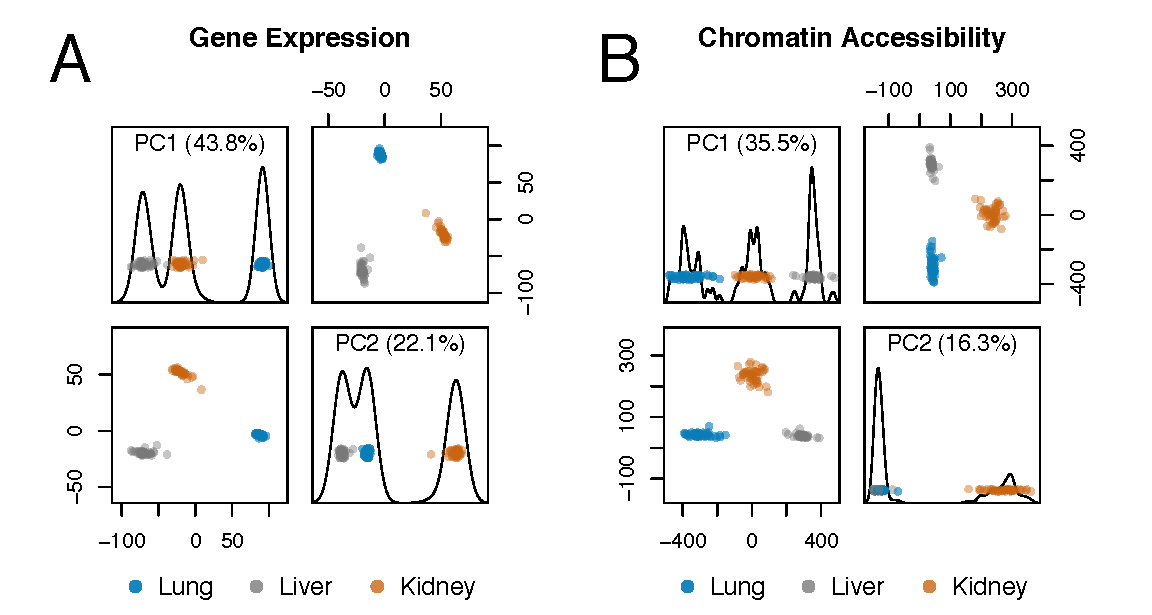
\includegraphics[width=0.8\textwidth, trim={0in 0in 0in 0in}, clip]{figs/pca_processed.pdf}
\caption{Principal components analysis of (A) gene expression and (B) chromatin accessibility for lung (blue), liver (gray), and kidney (orange) tissue samples derived from RNA-seq and ATAC-seq data respectively. Principal components (PCs) 1 and 2 capture a majority of the variance and show a greater amount of between tissue variability than within tissue variability. \label{fig:pca_plots}}
\end{figure*}

\begin{figure*}[hp]
\renewcommand{\familydefault}{\sfdefault}\normalfont
\centering
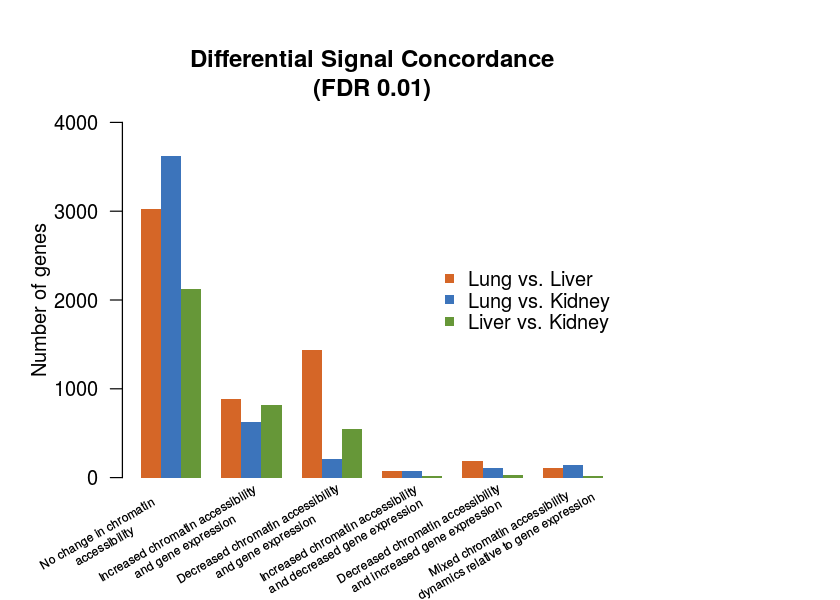
\includegraphics[width=0.8\textwidth, trim={0in 0in 0in 0in}, clip]{figs/diff_concordance.png}
\caption{Concordance between DE genes and DARs in between-tissue comparisons. DE genes were categorized by direction of DE and chromatin accessibility in their promoter regions.\label{fig:diff_concordance}}
\end{figure*}

\begin{figure*}[hp]
\renewcommand{\familydefault}{\sfdefault}\normalfont
\centering
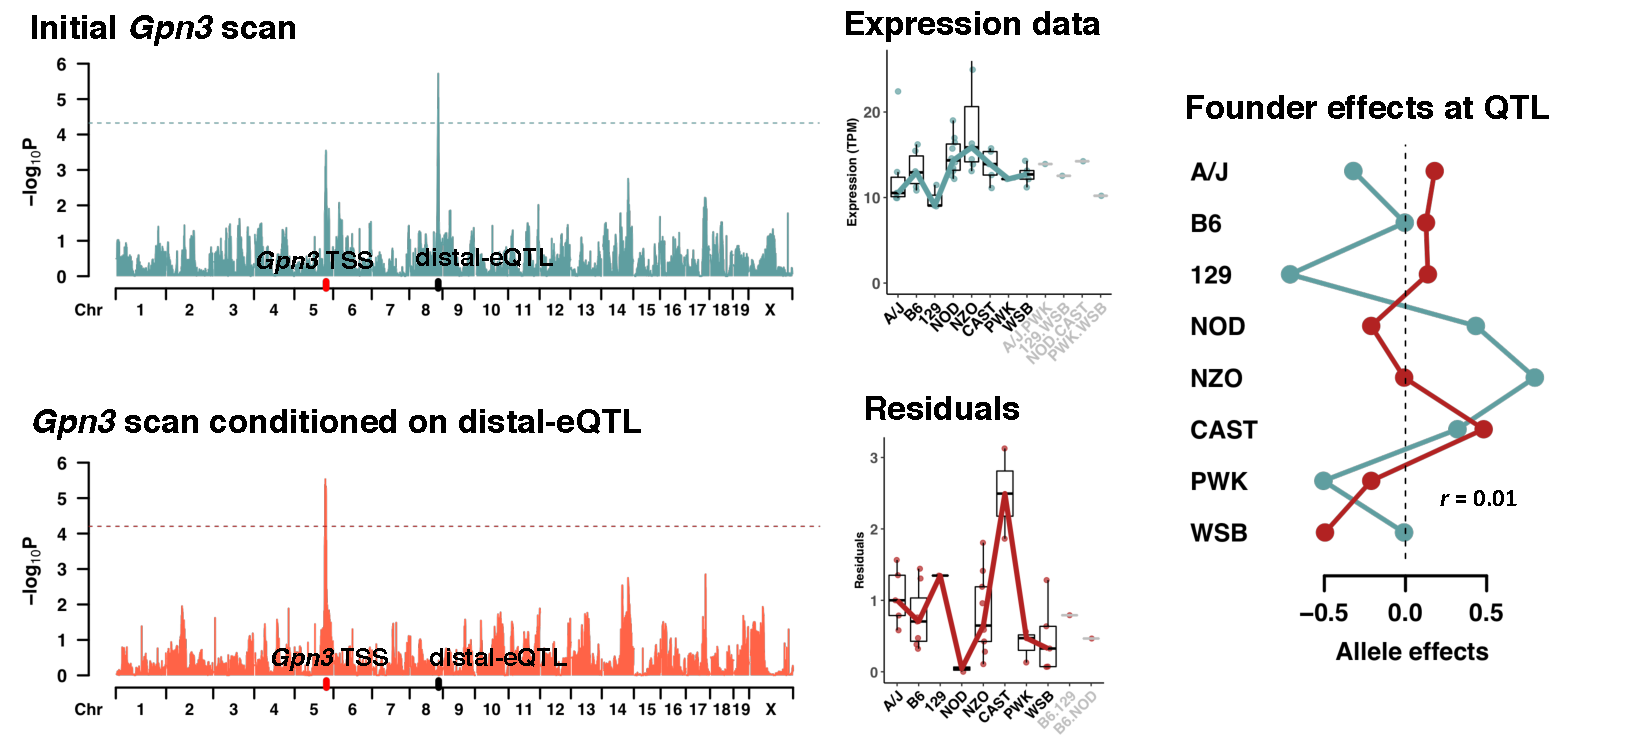
\includegraphics[width=\textwidth, trim={0in 0in 0in 0in}, clip]{figs/gpn3_conditional_scan.pdf}
\caption{\textbf{Detection of local-eQTL after conditioning on distal-eQTL.} The multi-stage conditional regression approach of Method 1 allows for the detection of multiple genome-wide significant QTL, which can then be appropriately incorporated into a FDR procedure across many outcomes. In this example in lung tissue, the gene \textit{Gpn3} initially has a strong distal-eQTL on chromosome 8 (A). Though a peak is detected near the TSS of \textit{Gpn3}, it does not meet genome-wide significance. However, after conditioning on the distal-eQTL, the local-eQTL is detected (B). Horizontal dashed lines represent empirical 95\% significance thresholds based on 1000 permutations.
\label{fig:conditional_scans}}
\end{figure*}

\begin{figure*}[h]
\renewcommand{\familydefault}{\sfdefault}\normalfont
\centering
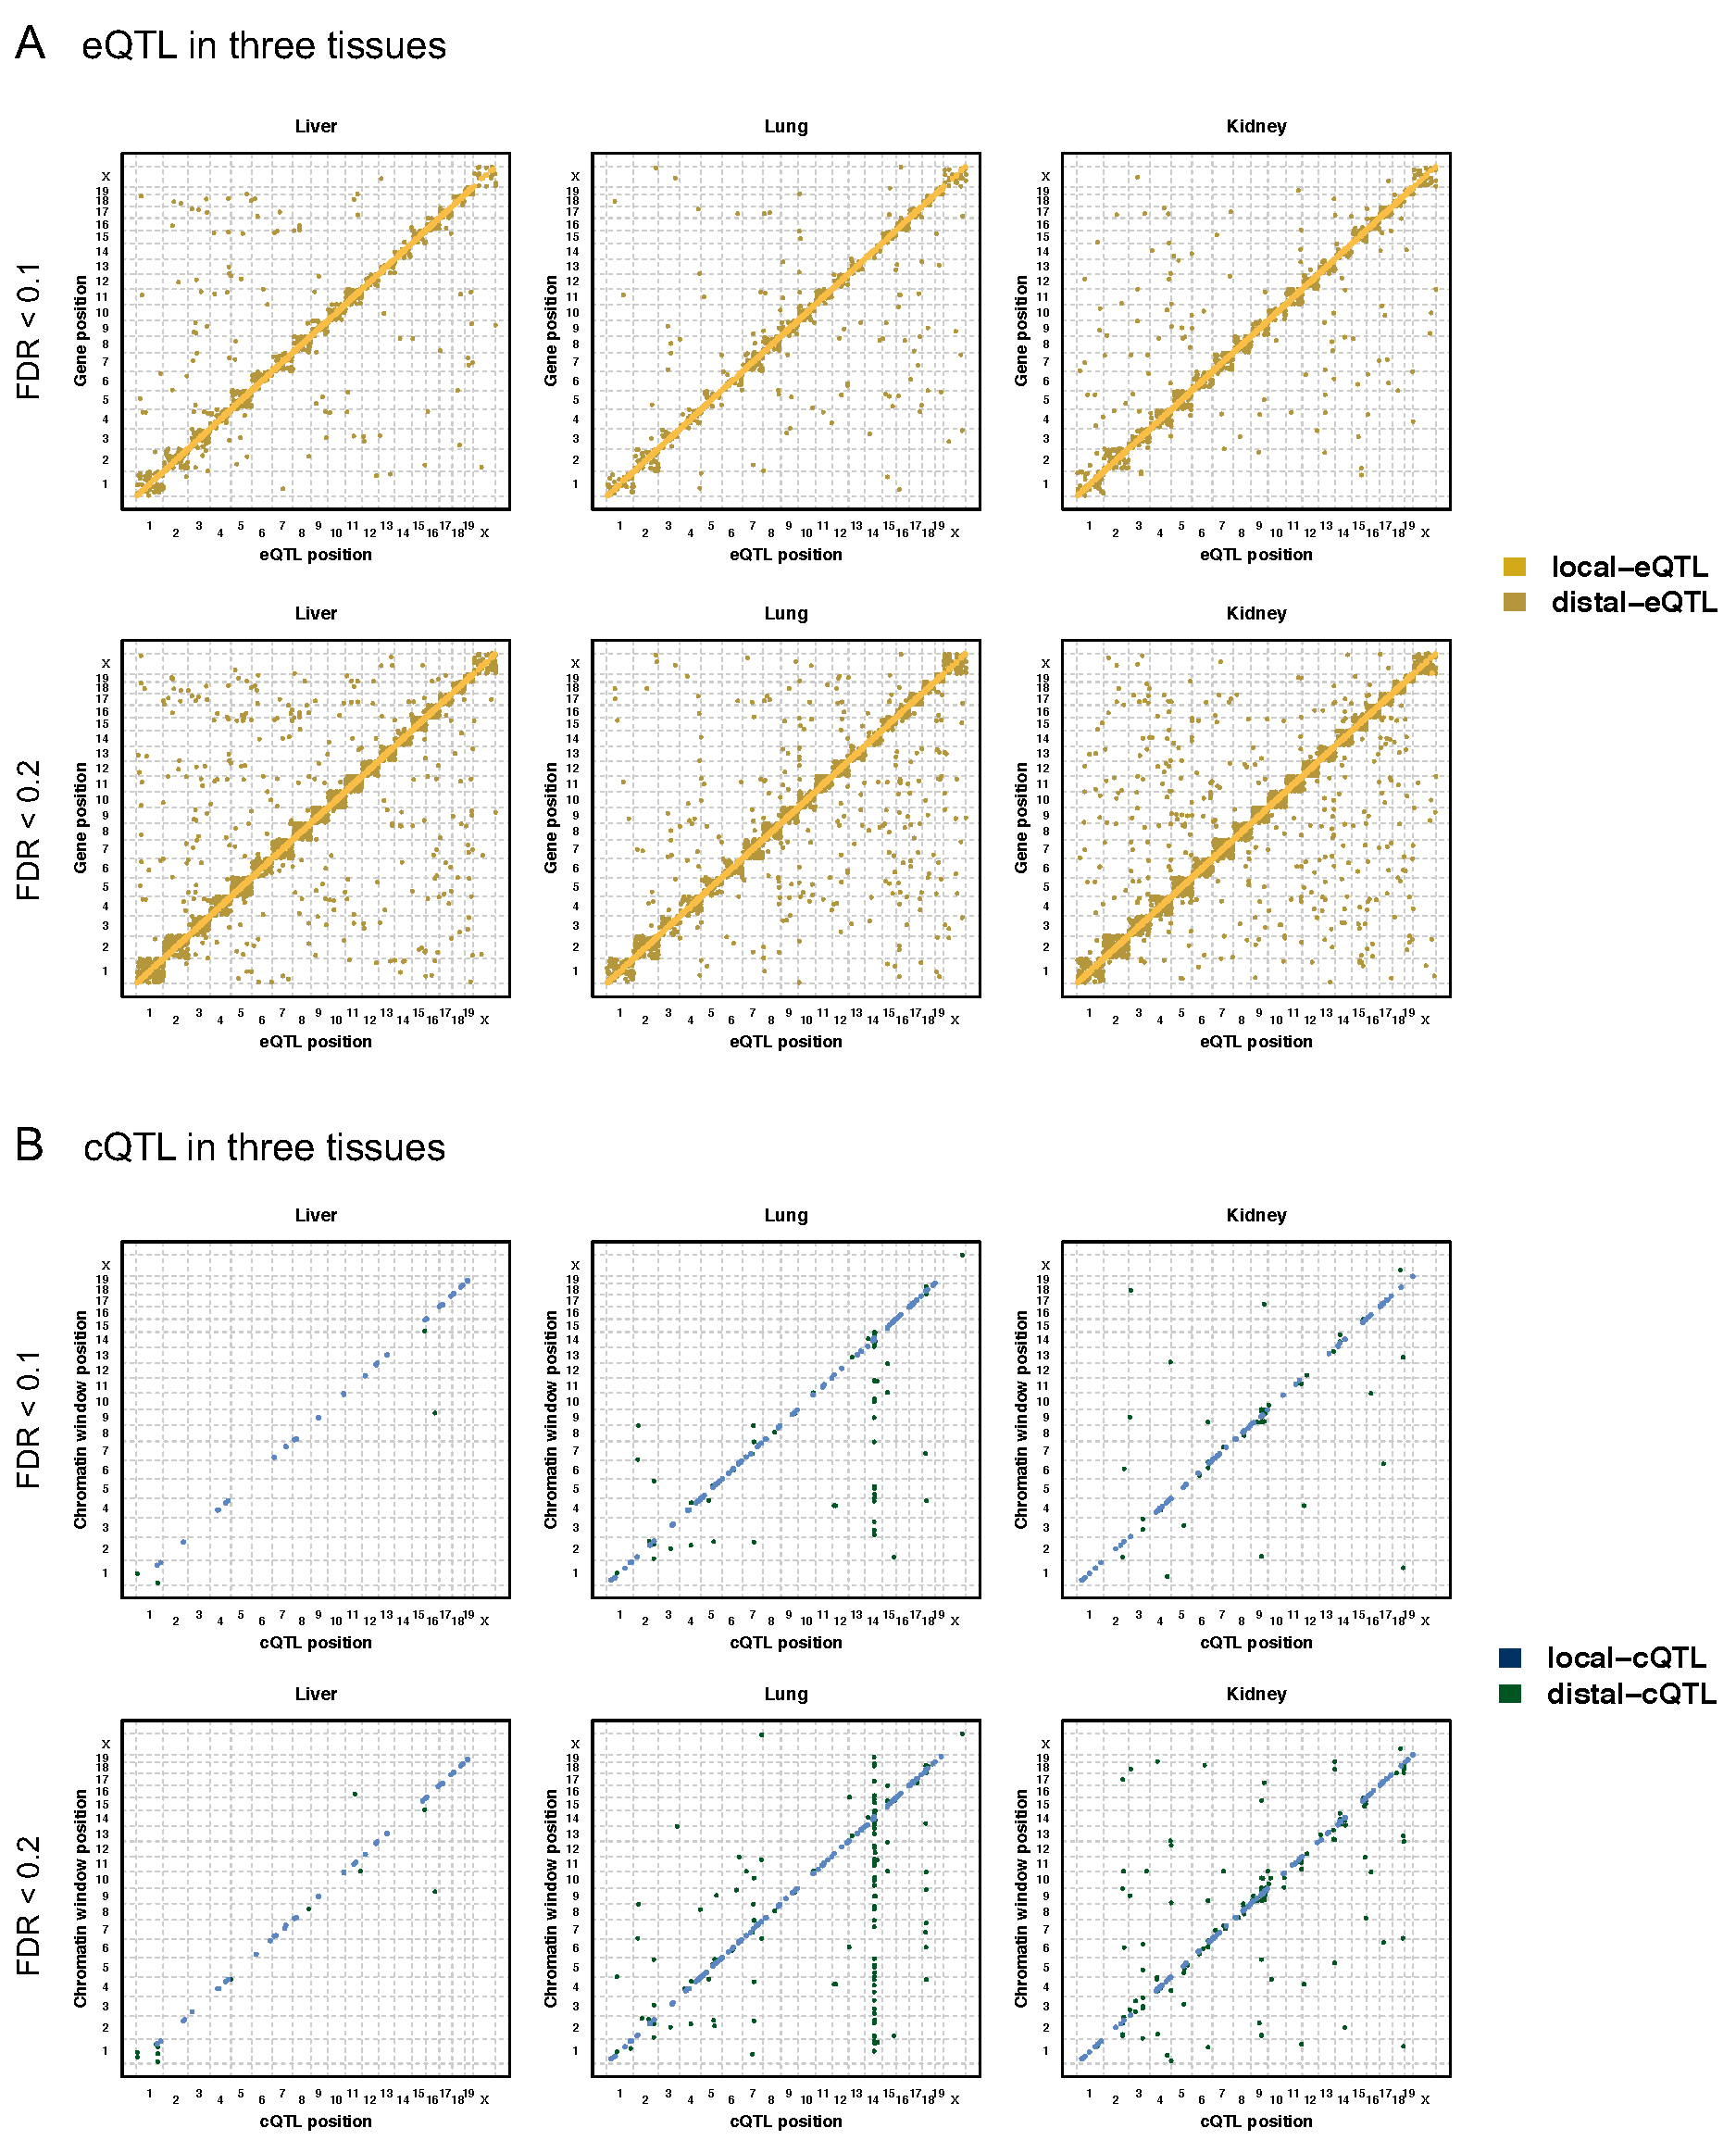
\includegraphics[width=0.8\textwidth, trim={0in 1.5in 0in 0in}, clip]{figs/qtl_map_supplemental.pdf}
\caption{\textbf{QTL mapping results using only Method 1 or Method 2.} QTL map plots of eQTL and cQTL with FDR controlled at 0.1 and 0.2 for liver, lung, and kidney. Detected QTL from Method 1 (multi-stage FDR) and Method 2 (chromosome-wide FDR) are included. Method 2, which uses FDR control for chromosome-wide significant QTL, produces a large number of intra-chromosomal distal QTL. The y-axis represents the genomic position of the gene or chromatin site, and the x-axis represents the genomic position of the QTL. Local-QTL appear as dots along the diagonal.
\label{fig:grid_fdr_plot}}
\end{figure*}

\begin{figure*}[h]
\centering
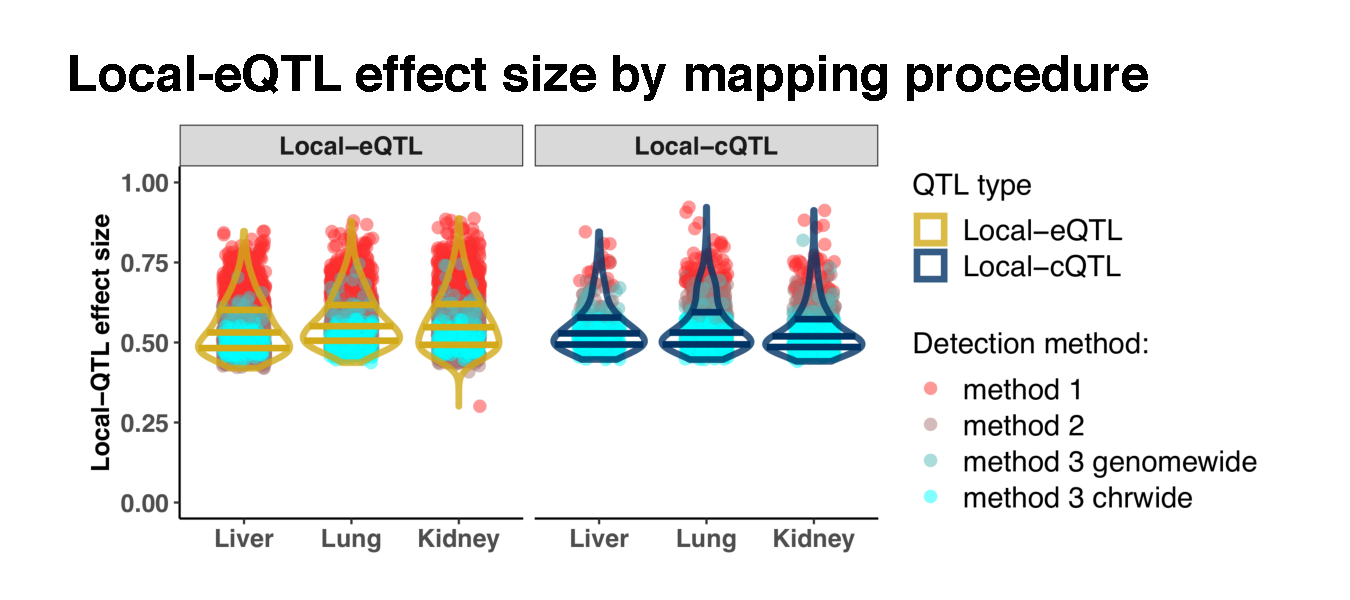
\includegraphics[width=0.85\textwidth, trim={0in 0in 0in 0in}, clip]{figs/qtl_effect_size_by_method.pdf}
\caption{\textbf{Local-QTL effect sizes by mapping procedure.} Statistical procedures with greater rigor have reduced power to detect QTL of smaller effect sizes, shown in liver, lung, and kidney tissues for gene expression (yellow line) and chromatin accessibility (blue line). Each dot represents a detected local-QTL, colored according to the highest stringency mapping procedure that detected it. The three horizontal bars represent the 25\textsuperscript{th}, 50\textsuperscript{th}, and 75\textsuperscript{th} quantiles of QTL effect sizes for all local-QTL per tissue. The multi-stage genome-wide FDR (Method 1) generally detects QTL with effect size > 30\%, whereas the chromosome-wide FDR (Method 2), and FWER-adjusted p-values (permP; Method 3), genome-wide or chromosome-wide can detect QTL effect sizes > 15\%. 
\label{fig:qtl_effect_sizes_by_method}}
\end{figure*}

\begin{figure*}[h]
\centering
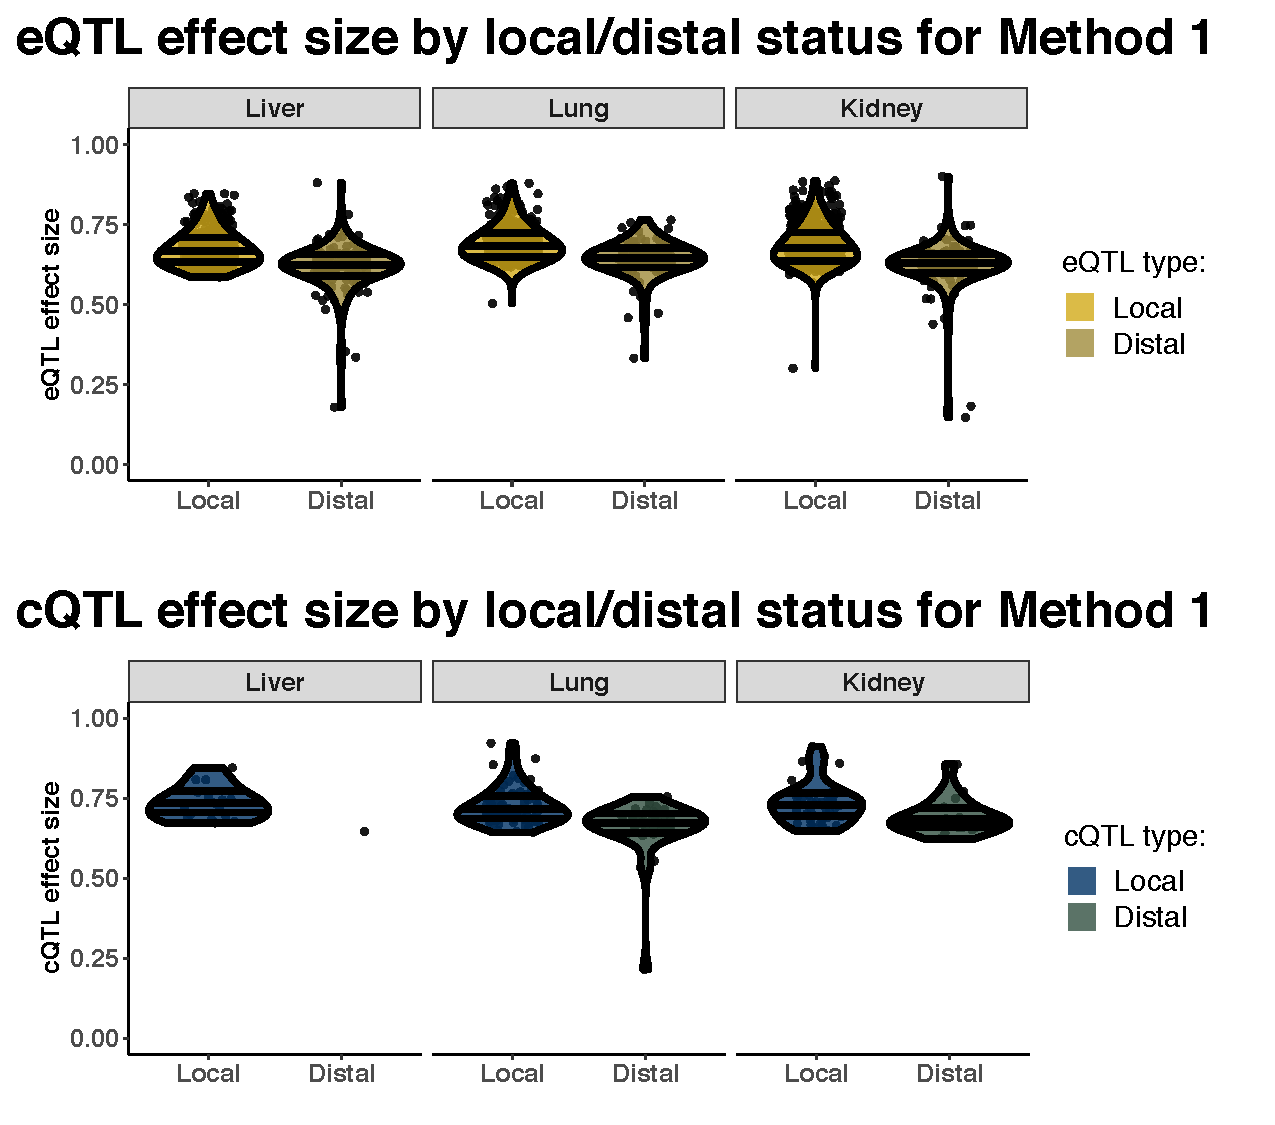
\includegraphics[width=0.75\textwidth, trim={0in 0in 0in 0in}, clip]{figs/qtl_effect_sizes_strict.pdf}
\caption{\textbf{QTL effect sizes by local/distal status for Method 1.} Each dot represents a detected QTL through either Method 1 (FDR $\leq$ 0.1). The three horizontal bars represent the 25\textsuperscript{th}, 50\textsuperscript{th}, and 75\textsuperscript{th} quantiles of QTL effect sizes for all local-QTL per tissue. More local-QTL are detected and have larger effects on average than the detected distal-QTL, in both gene expression and chromatin accessibility. 
\label{fig:qtl_effect_sizes_strict}}
\end{figure*}

\begin{figure*}[h]
\centering
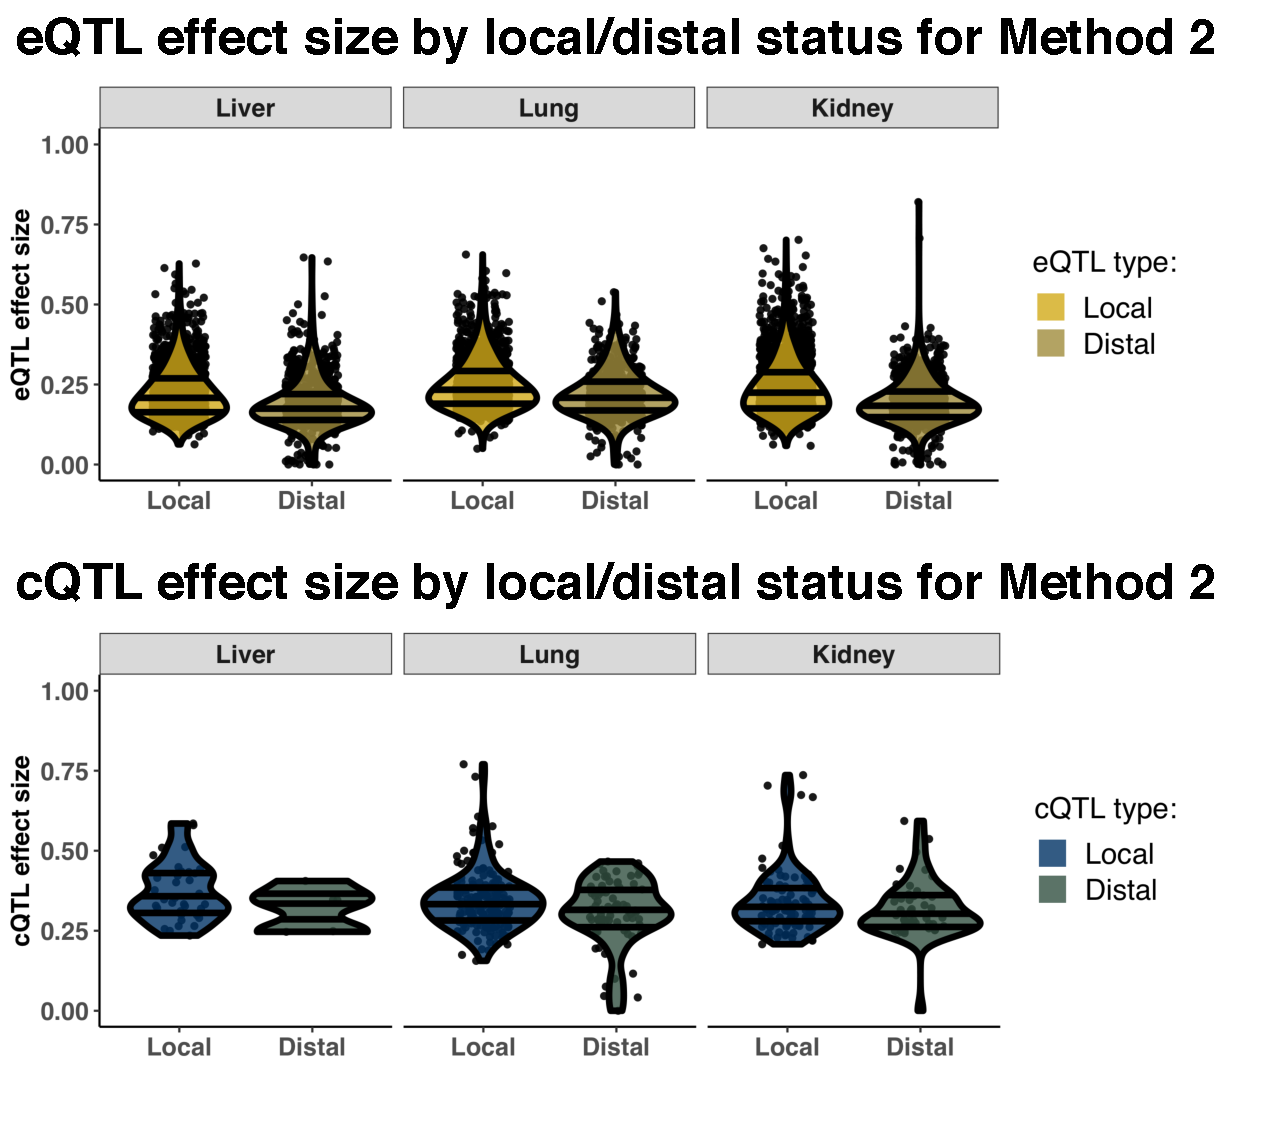
\includegraphics[width=0.75\textwidth, trim={0in 0.25in 0in 0in}, clip]{figs/qtl_effect_sizes_permissive.pdf}
\caption{\textbf{QTL effect sizes by local/distal status for Methods 1 and 2.} Each dot represents a QTL detected through either Method 1 or Method 2 (FDR $\leq$ 0.1).  The three horizontal bars represent the 25\textsuperscript{th}, 50\textsuperscript{th}, and 75\textsuperscript{th} quantiles of QTL effect sizes for all local-QTL per tissue. Consistent with Method 1 results, more local-eQTL are detected and have higher effects than distal-QTL. Method 2 detects a large number of intra-chromosomal distal-QTL that Method 1 does not, many of which have low effect sizes.
\label{fig:qtl_effect_sizes_permissive}}
\end{figure*}

\begin{figure*}[hp]
\renewcommand{\familydefault}{\sfdefault}\normalfont
\centering
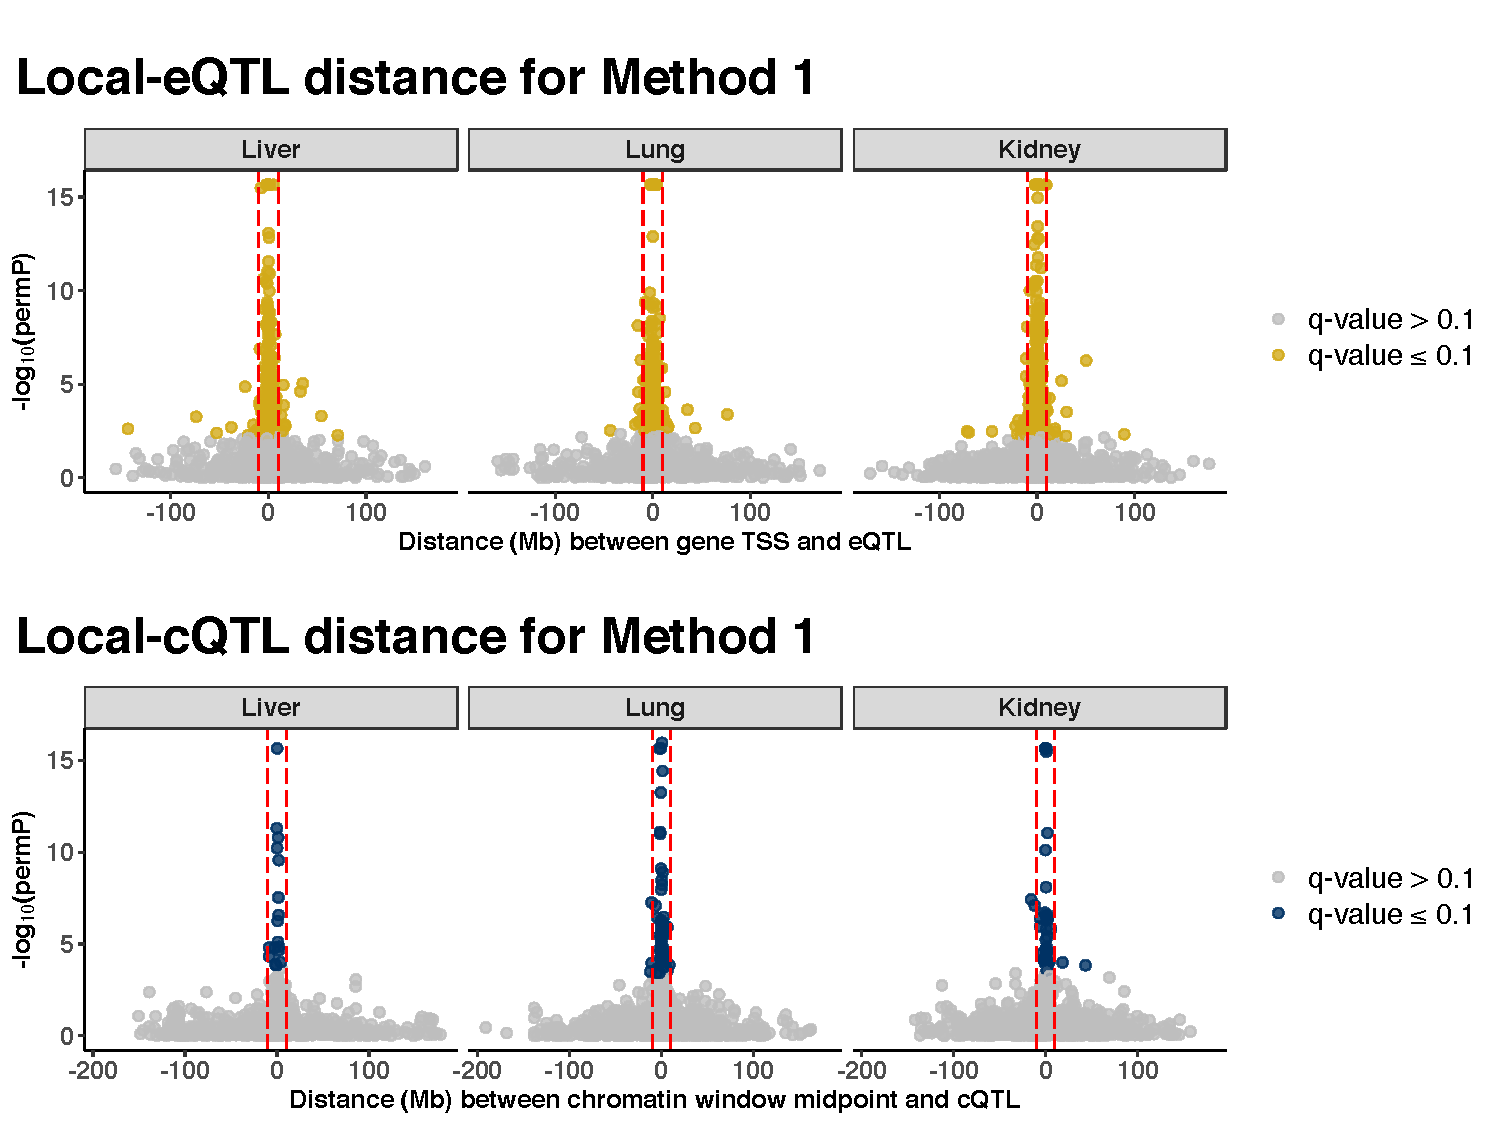
\includegraphics[width=0.75\textwidth]{figs/qtl_distance_method1.pdf}
\caption{\textbf{Highly significant QTL are proximal to gene TSS and chromatin window midpoint.} The genome-wide permutation-based p-value (permP) from Method 1 (first stage-only) for eQTL and cQTL compared to the distance (Mb) from the gene TSS and the midpoint of the chromatin site, respectively. Inter-chromosomal distal-QTL are not included. The red dashed lines represent 10 Mb upstream and downstream of the gene TSS or the midpoint of the chromatin site for classifying QTL as local or distal. Significant signals (yellow or blue), based on $\text{q-value} \le 0.1$, are largely local. \label{fig:genomewide_dist}}
\end{figure*}

\begin{figure*}[hp]
\renewcommand{\familydefault}{\sfdefault}\normalfont
\centering
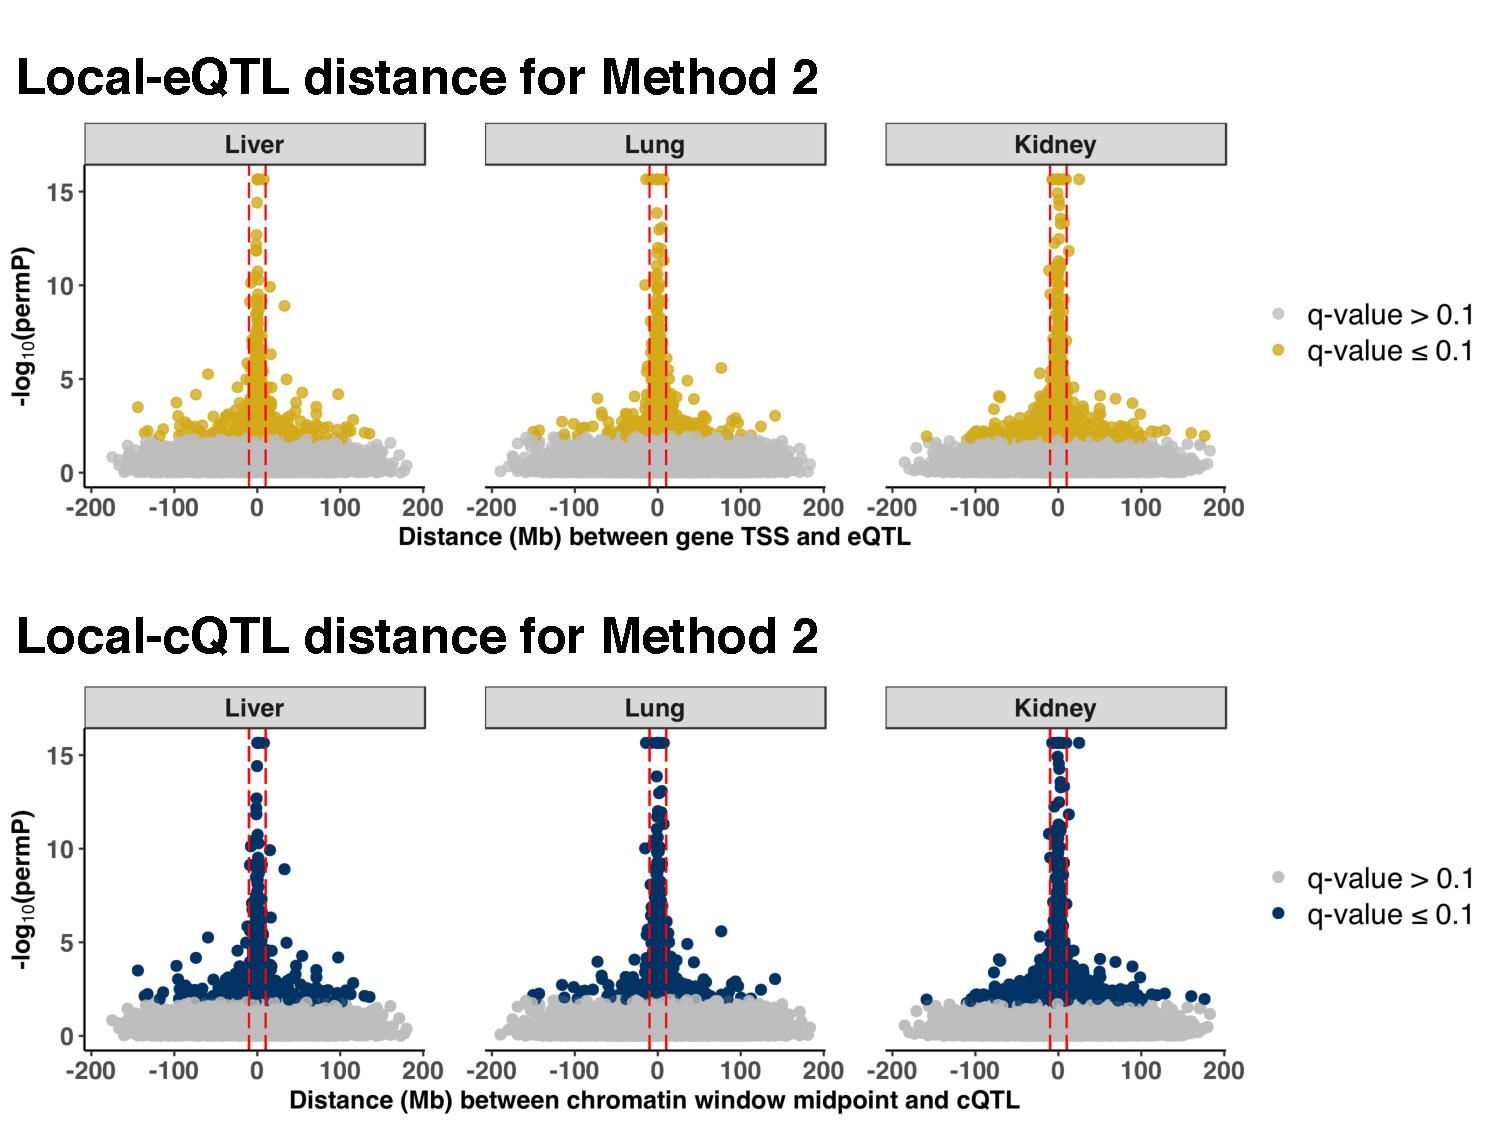
\includegraphics[width=0.75\textwidth]{figs/qtl_distance_method2.pdf}
\caption{\textbf{Methods that use chromosome-wide significance detect many putative intra-chromosomal distal-QTL.} The chromosome-wide permutation-based p-value (permP) from Method 2 for eQTL and cQTL compared to distance (Mb) from the gene TSS and the midpoint of the chromatin site, respectively. Method 2 is restricted to QTL on the local-chromosome. The red dashed lines represent 10 Mb upstream and downstream of gene TSS or chromatin site for classifying an association as local or distal. Significant QTL (yellow or blue) are largely proximal.
\label{fig:chrwide_dist}}
\end{figure*}

\begin{figure*}[hp]
\renewcommand{\familydefault}{\sfdefault}\normalfont
\centering
\includegraphics[width=0.9\textwidth, page=7, trim={2in 2in 2in 1in}, clip]{figs/tissue_comparison_figures.pdf}
\caption{Stuff.
\label{fig:eqtl_effects_abs}}
\end{figure*}

\begin{figure*}[hp]
\renewcommand{\familydefault}{\sfdefault}\normalfont
\centering
\includegraphics[width=0.9\textwidth, page=8, trim={2in 2in 2in 2in}, clip]{figs/tissue_comparison_figures.pdf}
\caption{Stuff.
\label{fig:cqtl_effects_abs}}
\end{figure*}

\begin{figure*}[hp]
\renewcommand{\familydefault}{\sfdefault}\normalfont
\centering
\includegraphics[width=0.9\textwidth, page=4, trim={2in 1in 2in 1in}, clip]{figs/tissue_comparison_figures.pdf}
\caption{Stuff.
\label{fig:qtl_effect_size_comparison}}
\end{figure*}

\begin{figure*}[hp]
\renewcommand{\familydefault}{\sfdefault}\normalfont
\centering
\includegraphics[width=0.9\textwidth, page=5, trim={2in 1in 2in 1in}, clip]{figs/tissue_comparison_figures.pdf}
\caption{Stuff.
\label{fig:qtl_cor_by_distance_comparison}}
\end{figure*}

\begin{figure*}[hp]
\renewcommand{\familydefault}{\sfdefault}\normalfont
\centering
\includegraphics[width=\textwidth, page=3, trim={3.5in 3in 3in 3in}, clip]{figs/tissue_comparison_figures.pdf}
\caption{Stuff.
\label{fig:qtl_pair_histograms}}
\end{figure*}

\begin{figure*}[hp]
\renewcommand{\familydefault}{\sfdefault}\normalfont
\centering
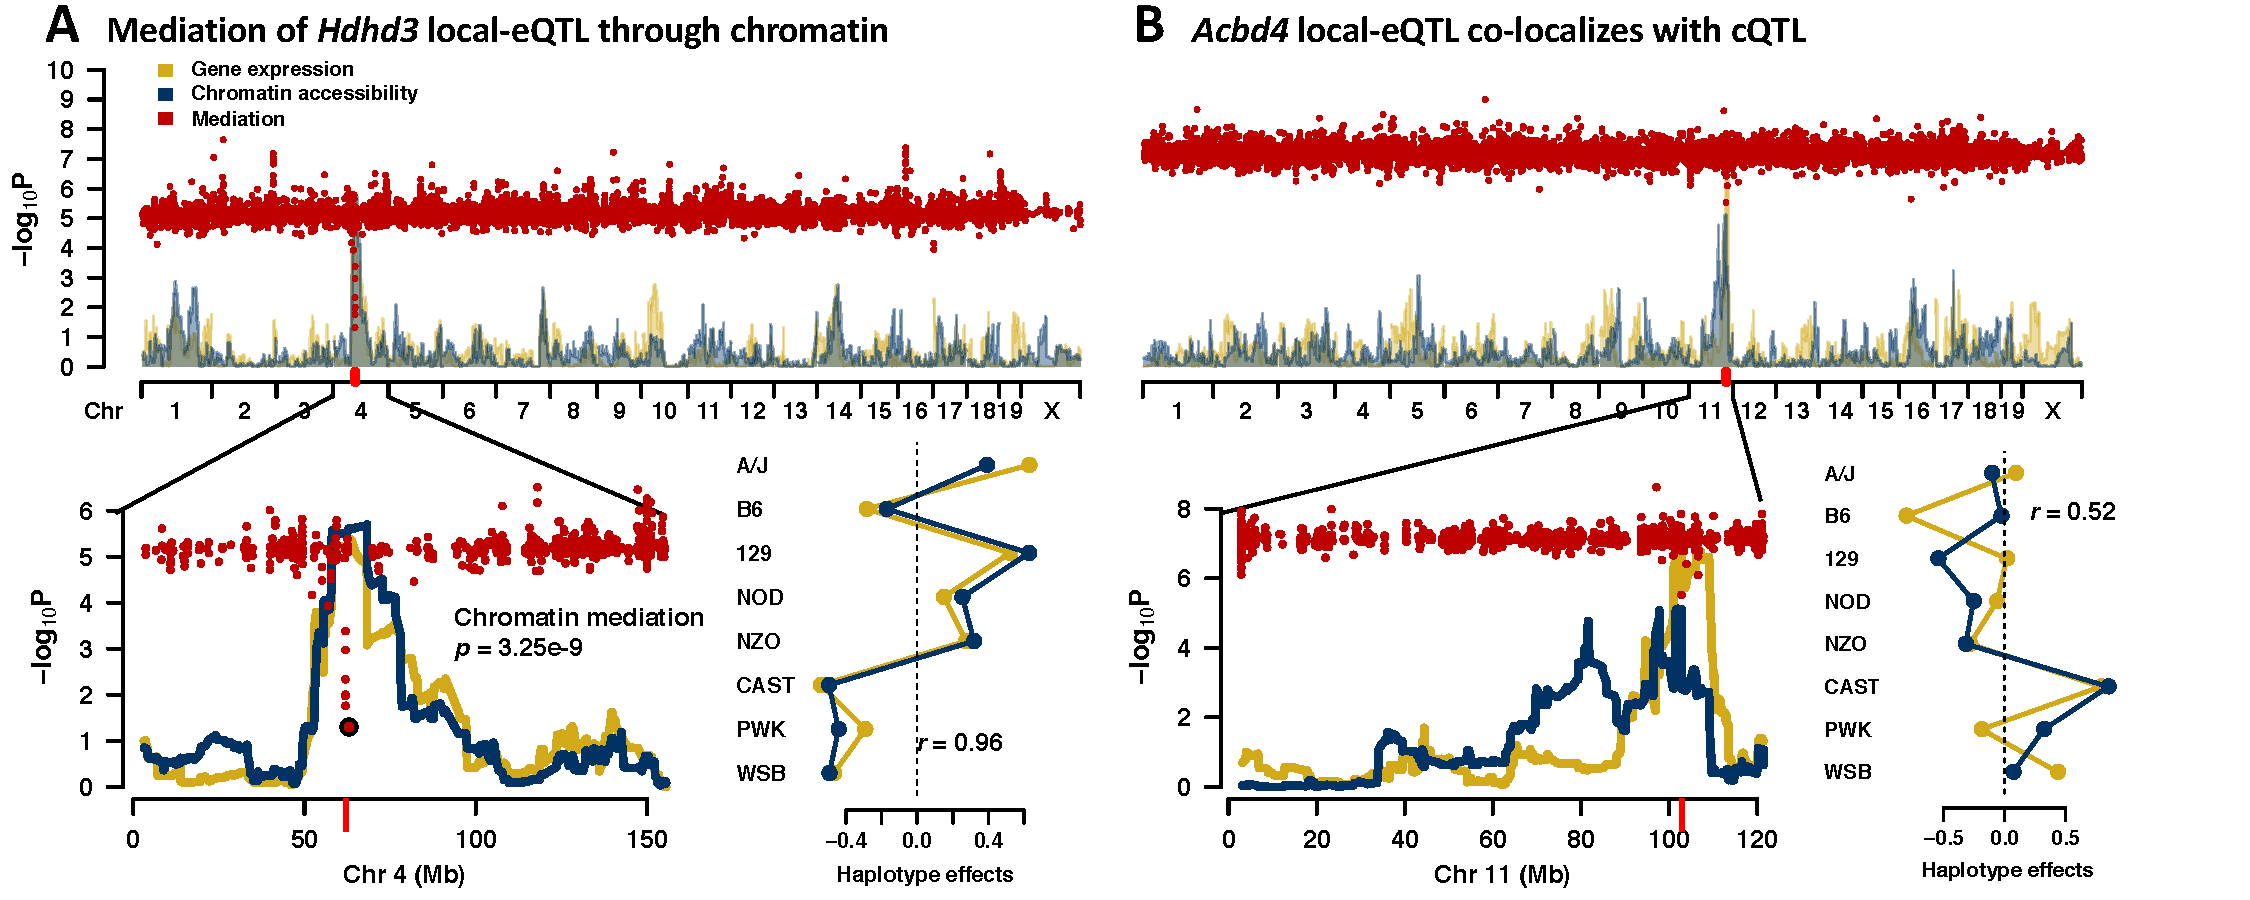
\includegraphics[width=\textwidth]{figs/mediation_or_colocal.pdf}
\caption{\textbf{Mediation of local-eQTL through chromatin state.} Detection of chromatin mediation requires that the eQTL and cQTL co-localize, as well as possess similar founder allele effects. Co-localizing cQTL are observed for local-eQTL for both \textit{Hdhd3} in liver tissue (A) and \textit{Acbd4} in kidney tissue (B). eQTL an cQTL scans are shown in the left plots. The red tick marks the TSS for both genes. Founder effects plots are in the middle. These effects are estimated as the centered and scaled regression coefficients. The effects for the eQTL and cQTL are highly correlated for \textit{Hdhd3} (B), but not for \textit{Acbd4} (E). Genome-wide eQTL, cQTL, and mediation are in the right column. Strong mediation of the eQTL through chromatin is detected for \textit{Hdhd3}, but not for \textit{Acbd4}. The effect size of the cQTL co-local to the \textit{Acbd4} is smaller than the eQTL, also inconsistent with the relationship depicted in \textbf{Figure \ref{fig:graph} A}.\label{fig:colocalization}}
\end{figure*}

\begin{figure*}[hp]
\renewcommand{\familydefault}{\sfdefault}\normalfont
\centering
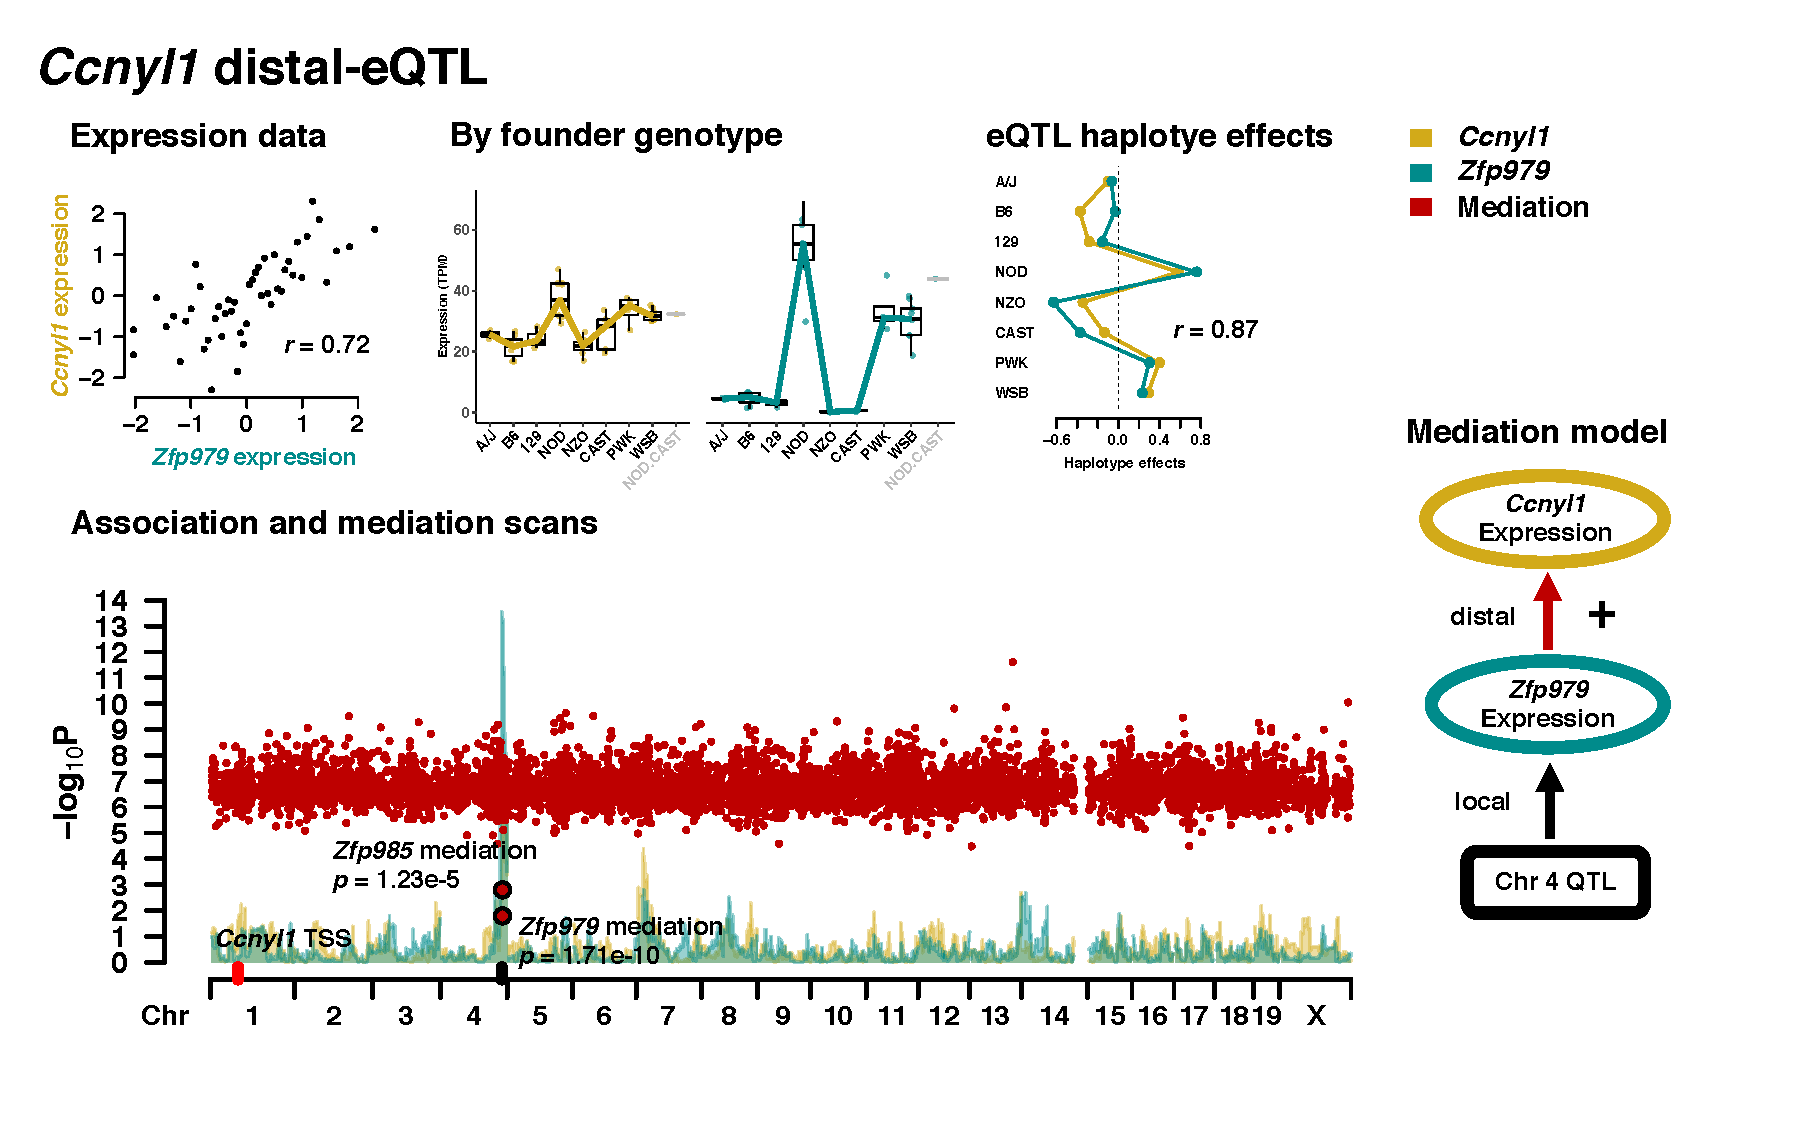
\includegraphics[width=\textwidth, trim={0in 0.5in 0in 0in}, clip]{figs/ccnyl1_mediation.pdf}
\caption{\textbf{Mediation of distal-eQTL of \textit{Ccnyl1}.} Distal-eQTL for one gene can correspond to local-eQTL of a mediating gene. The gene \textit{Ccnyl1}, located on chromosome 1, has a strong distal-eQTL on chromosome 4. Genes \textit{Zfp979} and \textit{Zfp985}, zinc finger proteins likely with DNA binding properties, are identified as strong mediators of the distal-eQTL, both genome-wide (A) and chromosome-wide (B). The founder haplotype effects for the distal-eQTL of \textit{Ccnyl1} are reduced but concordant with the effects the local-eQTL of \textit{Zfp979}, which is consistent with the relationship in \textbf{Figure \ref{fig:graph} B}.\label{fig:ccnyl1_exmediation}}
\end{figure*}


